% Dossier de conception
% Version 1.3

% Historique des versions
% 22/01/08 0.1 Version initiale
% 25/01/08 0.2
% 27/01/08 0.3
% 28/01/08 1.0 Première version presque complète, à étoffer
% 28/01/08 1.1 Version complète, à étoffer
% 03/02/08 1.2 Version toujours en cours...
% 05/02/08 1.3 À livrabiliser.

\documentclass[a4paper, 11pt, final]{article}

\usepackage[utf8]{inputenc} % Texte en utf-8
\usepackage[cyr]{aeguill} % Coupure des mots accentués
\usepackage[francais]{babel} % Typographie française
\usepackage[pdftex, hypertexnames=false, colorlinks=true, final]{hyperref}
\usepackage[final]{graphicx}
\usepackage{url} % Gestion des URLs
\usepackage{geometry}
\usepackage{fancyhdr}
\usepackage[Lenny]{fncychap}

% Marges à gauche et à droite de 3cm
\geometry{margin=3cm}

% Utilisation des headers et footers personnalisés de fancyhdr
\pagestyle{fancy}

% Images dans le dossier ./images/
\graphicspath{{./images/}}

% Gestion des métadonnées étranges à rendre visibles au rendu
\newcommand\docname{CCPv1.3}
\newcommand\docauthor{Guillaume Ayoub}
\newcommand\docstatus{LIVRABLE} % EN COURS, ATTENTE, VALIDE ou LIVRABLE

% Numérotation mieux
%\renewcommand\thechapter{\Alph{chapter}}
%\renewcommand\thesection{\Roman{section}}
%\renewcommand\thesubsection{\arabic{subsection}}
%\renewcommand\thesubsubsection{\alph{subsubsection}}

% Format de citation de références standard, marche avec quasiment tout
\newcommand\fullref[1]{\ref{#1}, page \pageref{#1}}

% En-têtes et pieds de page
\lhead{\docname}
\lfoot{Auteur : H4213}
\cfoot{}
\rfoot{\thepage}

% Titre du document maître
\title{\textbf{COPEVUE}\\
\rule{\textwidth}{1pt}{}\\
\Huge{\textsc{Dossier de conception}}}
\author{\docauthor{} (H4213)}
\date{\docname{} --- \today{} (\docstatus{})}

\begin{document}

\maketitle

\tableofcontents

\pagebreak

% Dossier de conception + Annexes : 20 pages maxi

% TODO:
% - Gestion de l'alimentation

\section{Introduction}
\subsection{Présentation du projet}
Il existe aujourd'hui de nombreux sites isolés et/ou difficiles
d'accès qui nécessitent une surveillance et parfois des actions à
distance. Ces sites se situent dans des espaces très différents tels
que les citernes placées dans les forêts escarpées du pourtour
méditerranéen, les réservoirs utilisés pour l'autonomie des chantiers
dans le grand Nord mais aussi les personnes âgées qui se retrouvent
souvent isolées.

Actuellement tous les contrôles et actions sont réalisés par un
opérateur qui doit se déplacer sur le site. Il n'y a donc que très peu
de réactivité, on ne peut pas avoir un suivi fin des évolutions et des
problèmes graves (par exemple la fuite d'un réservoir) ne peuvent pas
être traités rapidement.

\paragraph{Étude COPEVUE}
L'objet de l'étude est la mise en place d'un système générique de
surveillance et d'action à distance sur des sites isolés. Le système
devra être évolutif, autonome et fiable.

\subsection{Présentation du document}
Ce document~-- Dossier de conception~-- définit une architecture
générique applicative et technique, une architecture de communication,
un interfaçage des sites isolés avec le reste du système, une
interface de communication ou modèle de communication.

\subsubsection{Objectifs}
Voici les objectifs de ce document :
\begin{itemize}
\item Quels sont les objets manipulés
\item Quelles sont les données manipulées
\item Analyse transformationnelle de ces données
\item Description des stations locales et du système central
\item Dimensionnement
\item Analyse de la complexité
\end{itemize}

\subsection{Documents applicables et de référence}
\subsubsection{Documents applicables}
\begin{itemize}
\item Dossier de gestion de la documentation
\item Dossier de spécification technique des besoins
\item Dossier de faisabilité
\end{itemize}

\subsubsection{Documents de référence}
\begin{itemize}
\item Plan de référence du dossier de conception
\end{itemize}


\section{Règles de conception}

\subsection{Architecture générale}
Comme définie dans le dossier \emph{Spécification Technique des
Besoins}, l'architecture générale retenue permet en théorie d'assurer
tous les besoins du système à réaliser.

\begin{figure}[!htp]
\begin{center}
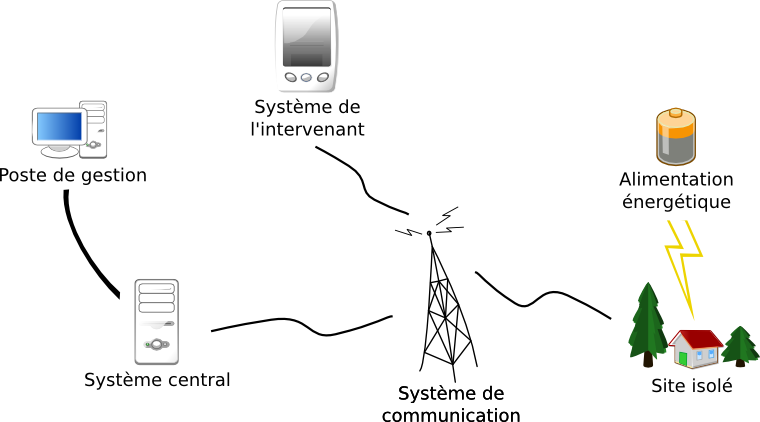
\includegraphics[width=.7\textwidth]{schema_architecture_generale.png}
\caption{Architecture générale}
\label{figure:schema_architecture_generale}
\end{center}
\end{figure}

Nous définissons dans ce \emph{Dossier de conception} les choix
techniques et logiciels possibles pour la réalisation du système
précédemment esquissé.

\subsection{Répartition des tâches}
Les sites isolés disposent d'un système capable de détecter, traiter
et faire suivre les informations nécessaires à la surveillance du
site. Ce système est composé d'un réseau CAN~-- pour la détection des
informations~-- couplé à un dispositif informatique embarqué~-- pour
le traitement et l'envoi des informations.

Les capteurs sont choisis pour leur robustesse et leur résistance aux
conditions extrêmes~-- hautes et basses températures, intempéries,
etc.

%Rémi:c'est nimp la suite non ? C'est pas le système de com' qui réveil le reste de l'appli? 
À un intervalle relativement court, une temporisation sur le site
isolé réveille le système de communication du site isolé qui
réveille à son tour l'ensemble du système embarqué. Le réseau CAN
reçoit les informations des capteurs, puis le système informatique
transmet ces valeurs au système embarqué pour le traitement.

Les traitements de données locaux ont pour principal but de détecter
des problèmes bénins que les actionneurs locaux peuvent résoudre
seuls. Les données sont alors stockées à court terme en attente d'une
récupération des informations par le système central. Il est en effet
profitable de détecter et résoudre ces imprévus sur place, puisqu'ils
évitent le déplacement coûteux d'un intervenant ; le système de
capteurs et d'actionneurs présent sur place pour les opérations
basiques~-- détection des niveaux et ouverture des silos dans notre
exemple~-- peut d'ailleurs s'avérer suffisant pour traiter ces
dysfonctionnements.

À un intervalle relativement long, une temporisation sur le système
central récupère les informations de capteurs, problèmes et
traitements locaux à des fins d'archivage et de statistiques.

Les problèmes urgents plus graves, qui ne peuvent pas être résolus
sans intervention humaine, sont détectés par le système isolé. Si une
intervention est nécessaire dans les plus courts délais, le système
isolé envoie un message au système central.

Ce message reçu et traité par le système central, la réponse du système central
dépendra de l'applicatif. Dans le cas de la Norvège, l'applicatif cherchera
l'intervenant le plus proche pour qu'il vienne intervenir sur le site.
Dans tous les cas, le système isolé se contente d'envoyer les données brutes
à la demande du système central. C'est alors le système central qui
détectera et traitera, à partir des données brutes qui lui sont
transférées, ces dysfonctionnements plus lourds. Par exemple, dans
le cas d'un problème grave, c'est le système central qui pourra
avertir un intervenant pour lui demander de résoudre le problème.

\paragraph{}
Le système central stocke et traite l'ensemble des données en
provenance des sites locaux~-- mesures et historique des
opérations. Ces traitements ont pour principal but de détecter les
problèmes nécessitant une intervention humaine sur site. Lors d'une
telle détection, les informations sur le problème sont stockées et un
message d'avertissement est envoyé aux personnes concernées par le
biais des moyens de communication internes du système~-- courriel par
accès Internet.

Les logiciels sur le serveur seront décomposés en modules afin d'offir
une conception en couches. La première couche sera constituée d'un
logiciel de bas niveau et d'un serveur de courriels. Le logiciel
récupère périodiquement les données des sites isolés et les stocke
sous forme de fichiers ; de plus, il fournit des services permettant
de récupérer les données à la demande, de commander les actionneurs
d'un site isolé et de configurer un site. Le serveur de courriels
permettra la communication entre le système central et les
intervenants. Les autres communications~-- récupération de données,
utilisation des actionneurs et configuration d'un site isolé par le
système central ou un intervenant~-- se fera par la mise en place d'un
accès distant sécurisé.

Au-dessus de cette couche se situera une application spécifique au cas
d'utilisation du système. Dans le cas de la Norvège, il doit permettre
l'optimisation de la logistique. Pour cela, il traitera les données stockées
et prendra les fichiers datant d'une durée dépendante de la requête~--
généralement d'une semaine à un an. Le système donnera alors une
analyse permettant de tirer de possibles améliorations. Toutes sortes
de calculs statistiques sont alors envisageables sur le même modèle
afin de répondre à d'éventuels besoins techniques, améliorer les
vitesses de traitement, réduire le nombre d'interventions humaines ou
optimiser les flux d'informations.

Les opérations de traitement statistique des données sont relativement
coûteuses en capacité de traitement et en accès disque, mais elles
restent rares et peuvent être lancées lors de faibles charges du
serveur. Le système central aura de plus à gérer peu d'accès
concurrentiels, ce qui en fait un système relativement simple à mettre
en place et à maintenir, puisqu'il n'est pas potentiellement soumis à
de fortes charges.


\section{Réseaux et connectiques}

\subsection{Réseau principal}
Entre les sites isolés et le système central, le principal flux
d'informations concerne l'échange des informations d'état du site.

Ces dernières années, une technologie utilisée pour l'échange des
données à longue distance s'est imposée : le GSM. À la base de la
grande majorité des réseaux de téléphonie mobile~-- tout du moins en
Europe~-- cette norme numérique performante et robuste semble toute
indiquée pour répondre à nos besoins. En effet, ses possibilités
techniques offrent les services adéquats sur des distances
raisonnables et son implantation importante indique une relative
simplicité d'utilisation tant pour les matériels disponibles que pour
les plateformes logicielles les supportant.

La principale limitation de cette solution technique est le mode de
transfert des données. Le GSM offre une allocation des ressources pour
tout le temps de la communication, alors qu'il nous faudrait, pour la
transmission de données, une allocation à chaque nouvelle transmission
afin de ne pas saturer les canaux de communication inutilement. Nous
nous tournons donc vers le GPRS, norme dérivée du GSM, qui permet de
pallier cette limitation. Notons également que la norme GPRS permet un
meilleur débit de données et donne la possibilité d'une connectivité
IP, requise dans notre cas d'utilisation.

\paragraph{}
La communication avec les sites isolés étant réalisée au travers d'un
réseau GPRS, il faut s'assurer qu'un tel réseau est disponible sur
place. Le déploiement d'un réseau privé est une opération coûteuse et
il faut privilégier au maximum l'utilisation des réseaux existants
appartenant aux opérateurs mobiles privés ou publics. Néanmoins, vu
l'isolement de la plupart des dispositifs, l'installation d'antennes
semble inévitable. Les zones en question n'étant pas urbanisées,
l'ajout d'antennes~-- si besoin surélevées par des pylônes~-- est à
prévoir. Tout comme les sites isolés, ces antennes devront être
autonomes et capables de résister aux intempéries.

La meilleure solution consiste à sous-traiter l'installation de ces
nouvelles antennes à un opérateur mobile. Un investissement partagé
nous permettrait d'investir de plus faibles sommes d'argent et de ne
pas avoir à assurer la maintenance. En contrepartie, l'opérateur
pourrait étendre son réseau à moindre coût et couvrir des zones peu
habitées. Il est également à noter que des subventions de l'Union
Européenne sont allouées à ce type d'installations.

\paragraph{}
Le réseau GSM/GPRS peut être également utilisé sur les systèmes
mobiles des intervenants extérieurs, qui peuvent avoir à administrer à
distance les installations des sites isolés. Un simple mécanisme
d'identification distante donne alors la possibilité d'interagir avec
les installations informatiques de ces sites et d'en prendre le
contrôle comme il serait possible de le faire sur place. Dans
l'éventualité d'un système isolé intègre, toutes les opérations sont
dès lors réalisables sans avoir à se déplacer physiquement sur site.

\subsection{Localisation}
Pour garder une vue d'ensemble du système, une localisation de chacun
des éléments du système doit être réalisée et actualisée en temps
réel si besoin est. On utilise pour ce faire le réseau actuel dédié à
cette tâche : le réseau GPS.

Dans le cas des éléments fixes~-- système central, poste de gestion et
sites isolés dans notre cas~-- il suffit d'une seule localisation à
l'installation du système, à l'aide d'une balise GPS simple. Cette
opération peut même être ignorée si un besoin de précision
d'emplacements ne se fait pas sentir.

Pour les éléments mobiles~-- majoritairement les \emph{smartphones}
des intervenants~-- une localisation en temps réel semble nécessaire à
des fins de vérification et de statistiques. On utilise alors les
possibilités GPS offertes par la plupart des \emph{smartphones}
présents sur le marché. Encore une fois, si le besoin n'est pas
présent, il est possible de se passer de cette fonctionnalité.

\subsection{Connectique de secours}
La connectique de secours permet à l'agent de sécurité de se connecter
directement au système embarqué en cas de panne du réseau
principal. Elle doit donc être fiable et facile à implémenter sur le
dispositif de l'agent et sur le système embarqué afin de limiter les
coûts de mise en œuvre.

La connectique USB, très répandue et éprouvée, permet une connexion
simple. Elle est disponible en standard sur un important nombre de
postes fixes et de \emph{smartphones}, et dispose de pilotes pour
plusieurs systèmes d'exploitation légers.


\section{Données et stockage}
Le choix du système de stockage des données, autant du point de vue
matériel que logiciel, est le point principal pour assurer la
pérennité des informations et pour en permettre un traitement
pertinent \emph{a posteriori}. On s'attachera au choix des
informations à stocker et sur les méthodes retenues pour ce stockage.

\paragraph{}
Le choix précis des données à stocker dépend de nombreux paramètres
aussi variés que le type de sites isolés à surveiller, les
optimisations que l'on veut réaliser, les calculs statistiques à
effectuer ou encore les contraintes légales. Les besoins peuvent même
évoluer au fil du temps selon les problèmes rencontrés. On peut
cependant lister un certain nombre d'évènements à archiver dans la
plupart des situations.

Tout d'abord, il faut absolument garder une trace des valeurs
principales envoyées par les sites isolés. Ces valeurs sont
indispensables à court terme pour décider des interventions humaines
et détecter de possibles problèmes~-- fuite sur un silo pour l'exemple
de la Norvège. À long terme, elles permettent assez facilement de mieux
planifier les interventions humaines et d'améliorer les différents
réglages sur l'ensemble des machines du réseau.

Il faut également archiver tous les problèmes intervenus sur
l'ensemble du réseau, que ce soit les problèmes bénins des sites
isolés, les erreurs informatiques de traitement ou de transmission
des informations, ou encore les problèmes à l'origine des
interventions humaines. Ces informations sont cruciales pour détecter
les problèmes récurrents et trouver les poins faibles du réseau.

Les informations stockées pouvant être variables, la structure des fichiers
qui contiennent ces informations sera elle aussi variable. Il faudra donc ajouter
pour chaque fichier une description de ce contenu. Vu que de nombreux fichiers
auront la même structure, on regroupera ces fichiers ainsi que leur description
dans un dossier commum.

\paragraph{}
D'un point de vue logiciel, les données sont archivées sur le système
central sous forme de fichiers texte afin de maintenir une
interopérabilité. Pour garder une certaine simplicité et efficacité de
parsage, on utilisera le XML. L'encodage des données se fait dans un
système de codage Unicode pour permettre le stockage d'informations
potentiellement dans la langue du client.

Nos données sont dès lors accessibles simplement sur tous les
systèmes, par un simple éditeur de texte au besoin. On assure la
pérennité des informations par l'utilisation d'un format standardisé
et éprouvé~-- le XML~-- sans pour autant hypothéquer les possibilités
de traitements complexes.

Dans la même optique d'interopérabilité, de simplicité et d'efficacité,
on utilisera des documents respectant la norme ISO~-- le DTD~-- afin de
décrire les fichiers XML.

D'un point de vue logique, le stockage des données peut suivre tout
ou partie du modèle conceptuel de stockage des données
OAIS\footnote{Modèle de référence pour un système ouvert d'archivage
d'information (OAIS) sur le site du CNES :
\url{http://vds.cnes.fr/pin/documents/projet_norme_oais_version_francaise.pdf}},
si le besoin de pérennité et de normalisation sont particulièrement
marqués.

\section{Architecture informatique}

\subsection{Architecture matérielle}
Le système central est choisi parmi les solutions offertes par un
grand constructeur afin de disposer d'une solution fiable et
maintenue. Les principaux besoins sont la fiabilité et la sécurité ; la
puissance de calcul n'a pas besoin d'être particulièrement élevée.

La capacité de stockage est choisie en fonction du nombre de mesures
récupérées ainsi que de la durée de stockage et de la nécessité de
duplication des données, par exemple pour un traitement extérieur ou
pour des raisons de sécurité.

\paragraph{}
Les intervenants sont équipés de \emph{smartphones}, qui nécessiteront
:
\begin{description}
\item[une connectique USB] pour une liaison filaire avec les sites isolés,
\item[une connectique GSM/GPRS] pour accéder aux possibilités de
  téléphonie et accéder à distance aux informations du système central
  et des sites à distance,
\item[une connectique GPS] pour suivre la position des intervenants à distance,
  celle-ci est optionnelle si le \emph{smartphones} dispose d'un système
  de géolocalisation par réseau GSM.
\end{description}

\paragraph{}
Les sites isolés sont surveillés par un système embarqué. Dans notre
cas, l'autonomie et la robustesse aux intempéries sont privilégiées
par rapport à d'autres facteurs qui ont une incidence moindre, tels
que la miniaturisation. Dans d'autres cas, comme par exemple la
surveillance des personnes âgées, la miniaturisation aurait cette fois
un rôle prépondérant alors que la robustesse aux intempéries aurait
alors peu d'incidence.

L'énergie est gérée par une carte minimaliste capable de réveiller les
autres composants en cas de problème, et suffisamment large pour
discuter avec le GPRS.

Le processeur central doit permettre le support des diverses
connectiques nécessaires~-- en particulier GPRS et USB. On peut par
exemple choisir un processeur ARM qui consomme très peu d'énergie
grâce à son bon ratio composants logiques/composants de contrôle.

\paragraph{}
L'alimentation en électricité de la station locale est l'un des points
les plus importants pour l'autonomie des sites. Il faut donc, au cas
par cas, être capable d'évaluer leur consommation. En fonctionnement,
cette consommation est environ cent fois plus élevé qu'en veille,
la fréquence et la durée des périodes d'activité du site isolé seront deux
facteurs déterminant de cette évaluation. De plus, la batterie doit être
suffisante pour maintenir l'alimentation entre deux interventions humaines
sur site, pendant lesquelles elle pourront être changées ou rechargées.
Le choix de la capacité des batteries se fera donc selon ces deux critères.

La batterie doit prévoir une marge de sécurité afin que la charge soit
toujours suffisante pour appliquer toutes les procédures d'urgence et en
informer le système central.

Si une batterie de taille suffisante est difficile à fournir ou si le site
est particulièrement adapté, on peut imaginer un système de production
d'appoint basé sur les énergies renouvelables comme une éolienne génératrice,
des panneaux photo-voltaïques ou un alternateur hydroélectrique qui se chargeront
de recharger la batterie de manière autonome.

\paragraph{}
Il faut également installer un poste qui sert à administrer le système
central. Ce poste peut se connecter et configurer le système central,
son architecture matérielle peut donc ressembler à celle d'un poste de
travail standard bas de gamme.

\subsection{Architecture logicielle}
Pour le système central, l'applicatif ne souffre que de peu de
contraintes techniques et laisse un choix assez large. Cependant,
certaines architectures offrent un panel plus large d'outils et de
garanties bénéfiques pour notre application.

Le serveur doit gérer deux applicatifs, l'un pour la réception et le
stockage, le second pour le traitement des données des sites, la
planification des interventions et effectuer tous les calculs
statistiques. Le système doit aussi supporter un serveur Web, serveur
qui doit permettre la gestion de pages dynamiques mais ne doit générer
que peu de connexions simultanées, ainsi qu'un serveur de courriels.

Ainsi, on se tourne vers un système basé sur FreeBSD, qui allie de
nombreux avantages tels que la possibilité d'administration à distance
-- \textit{via} SSH~-- la robustesse, la sécurité, la rapidité et la
gratuité de licence. On tire également bénéfice de l'architecture UNIX,
normalisée et utilisée par bon nombre de systèmes d'exploitation.

\paragraph{}
Le système embarqué des sites isolés doit fonctionner avec un système
petit et peu gourmand en ressources, qui doit supporter la veille et
l'hibernation si possible afin d'économiser l'énergie. Le système doit
également ne pas être un frein au support des connectiques nécessaires
-- USB et GSM/GPRS. La gestion de certains protocoles réseaux comme
SSH est également requise.

Le seul système d'exploitation à fournir ces possibilités est
TinyOS\footnote{Présentation de TinyOS sur l'encyclopédie Wikipédia :
\url{http://fr.wikipedia.org/wiki/TinyOS}}. Malgré son jeune âge, il
est particulièrement complet et suffisamment robuste pour gérer nos
sites isolés.

\section{Sécurité}
Le transfert des données est l'élément critique du système quant à
leur sécurisation. Il est donc crucial de concevoir un réseau dont
chacun des maillons est parfaitement hermétique et ne pourra pas être
piraté ni espionné par un élément extérieur.

\subsection{Sites}
Dans notre système, un seul site stocke les informations : le site
central. En effet, tous les autres sites par lesquels passe
l'information~-- le site isolé et le système des intervenants~-- ne
doivent pas stocker cette information. Le système isolé se contente de
traiter les informations et de les renvoyer au système central, et le
système des intervenants peut consulter les informations \emph{via}
les protocoles d'accès à distante sans jamais les rapatrier sous forme
de fichier pérenne.

\paragraph{}
Le site central doit donc être le site où se concentre la
sécurisation.

Le premier élément à sécuriser du site est le système d'exploitation,
la couche applicative la plus basse. Les systèmes BSD sont reconnus
pour leur sécurité et font office de références en ce qui concerne la
robustesse face aux attaques, non seulement vis-à-vis du
noyau mais aussi pour les paquets applicatifs fournis par défaut, en
particulier les couches réseau et le serveur Apache.

Les applications qui s'appuient sur le noyau, c'est-à-dire les
différents serveurs disponibles, sont généralement les points noirs de
la sécurité. Cependant, dans le cas des distributions BSD, ces
serveurs et leur intégration sont méticuleusement scrutés pour
garantir un haut niveau de protection et un nombre de failles
particulièrement bas. De plus, le système de paquetages permet une
mise à jour aisée et par conséquent un niveau de sécurité
particulièrement élevé.

Le serveur Web Apache et le serveur d'accès distant OpenSSH sont les
principaux logiciels susceptibles d'être accessibles depuis
l'extérieur et de ce fait potentiellement vulnérables. Le faible
nombre de failles de sécurité et la rapidité de leur correction en
font pourtant des outils parmi les plus fiables du marché, et l'on
peut sans hésitation les utiliser dans une politique de sécurité.

\paragraph{}
On veille tout de même à la sécurisation des autres sites ayant accès
à l'information. Si les risques d'espionnage de ces sites sont
relativement restreints et leur utilité limitée, il convient tout de
même d'en assurer une certaine robustesses afin d'éviter les attaques
les plus courantes.

\subsection{Réseaux}
La sécurité des réseaux va s'appuyer en très grande partie sur la
sécurité des protocoles utilisés et sur leur capacité à rendre les
données inaccessibles aux machines auxquelles elles ne sont pas
destinées.

\paragraph{}
Le réseau GSM, tout d'abord, est utilisé pour le transfert des données
entre les sites isolés et le système central. Cette norme ne crypte
pas les données, les rendant en théorie récupérables par n'importe
quelle machine capable d'espionner le réseau. Elle repose cependant
sur le TDMA\footnote{Présentation de TDMA sur l'encyclopédie Wikipédia
: \url{http://fr.wikipedia.org/wiki/TDMA}.}, un mode de multiplexage
temporel rendant l'assemblage des paquets composant la communication
assez complexe pour qu'on la considère impossible. On peut, de ce
fait, décemment considérer ce réseau comme insensible aux attaques
d'espionnage ou de type \emph{man in the middle}.

\paragraph{}
Les autres transferts d'informations se font sur le réseau
ethernet. Sur ce réseau, les différents échanges passent tous par une
couche SSL\footnote{Présentation de SSL sur l'encyclopédie Wikipédia :
\url{http://fr.wikipedia.org/wiki/SSL}.}, que ce soit par le biais des
protocoles SSH ou HTTPS. La couche SSL se charge de sécuriser les
données échangées par diverses méthodes d'authentification et de
chiffrage, il est donc en pratique très complexe voire impossible de
récupérer les informations transmises. Quelques attaques très rares
ont abouti par le passé pour contourner SSL, mais elles sont restées
marginales et les failles incriminées ont été facilement et rapidement
réparées.

\section{Démarrages et arrêts, gestion des erreurs}
L'ensemble des parties du système doit être, dans un fonctionnement
normal et optimal, en fonctionnement et prêt à l'emploi. Les taux de
disponibilité des machines doivent être maximaux. On remarquera tout
de même une tolérance à certaines indisponibilités dans la section de
gestion des erreurs~-- voir
\fullref{subsection:erreurs_et_indisponibilites}.

Seuls les sites isolés, pour des contraintes d'économie d'énergie, ont
un fonctionnement particulier : l'ensemble du système isolé, hormis
les gestionnaires de communication, est en hibernation. Les composants
de traitement et de détection de l'information ne sont alimentés que
lorsqu'une demande est formulée de la part du système central
\emph{via} le réseau GSM ou de la part d'un intervenant technicien
\emph{via} USB. Le composant de communication alimente à nouveau
l'ensemble du système pour récupérer et traiter les informations.

\subsection{Démarrages et arrêts des différentes parties du système}
Le premier élément à intégrer au système est le système central,
véritable chef d'orchestre de l'ensemble. Après l'avoir connecté aux
différents systèmes de communication~-- GSM et ethernet~-- il reste à
démarrer les serveurs Apache et SSH, puis à lancer les deux logiciels
de récupération et de traitement des résultats.

On peut alors installer le poste de gestion, dont le seul but est
d'administrer le système central. Ce poste n'est pas crucial dans
l'ensemble de l'architecture, mais il est nécessaire pour intervenir
rapidement sur le système central en cas de panne.

Sur cette architecture, on peut dès lors connecter les systèmes des
intervenants, qui ont accès aux applicatifs serveurs du système
central et des futurs sites isolés.

Enfin, on ajoute des sites isolés indépendants les uns des autres. Sur
site, il est nécessaire de connecter les systèmes embarqués aux
réseaux de communication, puis de démarrer les applicatifs serveurs et
les différentes temporisations. Du côté du système central, on doit
prendre en compte ce nouveau site dans l'ensemble des sites à
surveiller.

\subsection{Gestion des erreurs et des indisponibilités}
\label{subsection:erreurs_et_indisponibilites}
L'architecture globale du système, faite de modules relativement
indépendants, offre une certaine tolérance aux erreurs et aux
indisponibilités sans avoir à ajouter une couche applicative
supplémentaire dédiée à cette gestion. Il est néanmoins nécessaire
d'ajouter à cette architecture une gestion intelligente de ce genre de
problèmes.

\paragraph{}
Certains éléments sont passifs et n'ont pas besoin d'une haute
disponibilité ; c'est typiquement le cas du poste de gestion ou du
système des intervenants, sur lesquels ne tourne aucun applicatif de
type serveur.

Dans le cas du premier, il n'est nécessaire d'avoir un système
opérationnel que lorsque l'on veut administrer le système central. Le
poste de gestion ne sert alors que de terminal pour cette
administration. Une disponibilité maximale devient alors inutile,
hormis dans certains cas qui sortent des limites de notre
conception~-- installation d'outils de surveillance à distance,
politique sécuritaire extrême avec accès au système central uniquement
par le poste de gestion, etc.

Dans le cas du second, la disponibilité des machines doit correspondre
avec la disponibilité des intervenants. Ici également, la machine ne
joue que le rôle de client et il n'est en théorie pas indispensable
qu'elle fonctionne à temps complet. Cette disponibilité influe
pourtant sur la rapidité d'intervention en cas de problème grave ; il
faut donc, tant que faire se peut, que les intervenants puissent être
joints rapidement et gardent par conséquent leur système disponible.

\paragraph{}
La disponibilité maximale du site distant est l'objectif même de notre
système. Leur architecture leur garantit une grande tolérance aux
fautes, notamment grâce au triplement des systèmes critiques~--
communication, acquisition, etc. Ainsi, le système sera
toujours disponible malgré l'arrêt d'un capteur ou la perte de la
connexion GPRS. En l'absence de connexion directe avec le serveur
central, le site isolé sera aussi capable de gérer de manière
autonome un certain nombre d'anomalies. Bien entendu, même si cette
robustesse permet un certaine souplesse dans le traitement de ces
indisponibilité partielles, leur réparation doit être intégrée
rapidement à planning de maintenance optimisé. Dans le cas contraire,
l'aggravation du problème ou le manque de visibilité risque
d'entraîner des erreurs plus graves entraînant une indisponibilité
complète nécessitant une maintenance d'urgence hors planning.



\paragraph{}

Le système de communication est le système nerveux de notre
application, son bon fonctionnement est indispensable pour permettre
aux acteurs de communiquer entre eux. Le contrat nous liant à
l'opérateur du réseau GRPS devra contenir une clause de maintenance
rapide.  Pendant toute la durée d'indisponibilité, les intervenants
devront faire le lien entre les sites distants et l'office des forêts
grâce à la connectique de secours. Les sites distants, isolés pourront
aussi compter sur leurs règles de gestion automatique pour effectuer
un certain nombre d'actions de routine de leur propre initiative.

Le système central est un élément indispensable de l'application,
toute indisponibilité de sa part empêche les activités de
planification et de détection rapide des alertes humaines. Cependant,
la récupération régulière des informations et le traitement des
problèmes bénins sont toujours réalisés par les sites distants. Une
indisponibilité courte ne devrait donc pas avoir d'incidence~-- la
durée correspondant à cette indisponibilité acceptable dépend bien sûr
de l'ordre de grandeur des opérations sur le système.

En cas d'indisponibilité durable du système central, l'ancien système
de relevé manuel devra être utilisé pour garantir la disponibilité des
sites distants. Des sauvegardes régulières et un contrat de
maintenance rapide seront donc indispensables pour limiter la durée
des pannes sur le système central.


\end{document}
